\documentclass[]{article}

%\usepackage{epcc}
\usepackage{jmlr2e}
%\usepackage[hyphens]{url}
%\PassOptionsToPackage{hyphens}{url}
%\usepackage[colorlinks=false, hidelinks]{hyperref}
\usepackage{amsmath}
\usepackage[toc,page]{appendix}
\usepackage[table]{xcolor}
\usepackage[marginparsep=30pt]{geometry}
\usepackage{stmaryrd}
\usepackage{algorithm}
\usepackage{algorithmic}
\usepackage{tikz}
\usepackage{pgfplots}
\usepackage{tabu}
\usepackage{longtable}
\usepackage{tabularx}
\usepackage{listings}
\usepackage{fancyref}
\usepackage{relsize}
\usepackage{float}
\usepackage{graphicx}
\usepackage{subcaption}
\usepackage{diagbox}
\usepackage{multirow}
\usepackage{slashbox}
\usepackage{graphics}
\usepackage{booktabs}
\usepackage{natbib}
\usepackage{csquotes}

\usetikzlibrary{%
    arrows,
    arrows.meta,
    decorations,
    backgrounds,
    positioning,
    fit,
    petri,
    shadows,
    datavisualization.formats.functions,
    calc,
    shapes,
    shapes.multipart,
    matrix,
    plotmarks
}

\usepgfplotslibrary{fillbetween, statistics, dateplot}

\pgfplotsset{%
  compat=1.3,
  every non boxed x axis/.style={%
  enlarge x limits=false,
  x axis line style={}%-stealth},
  },
  every boxed x axis/.style={},
  every non boxed y axis/.style={%
  enlarge y limits=false,
  y axis line style={}%-stealth},
  },
  every boxed y axis/.style={},
}

\renewcommand{\labelenumii}{\theenumii}
\renewcommand{\theenumii}{\theenumi.\arabic{enumii}.}

\bibliographystyle{plainnat}
\bibpunct{(}{)}{;}{a}{,}{,}

\newenvironment{declaration}
{\centerline{\large\bf Declaration}\vspace{0.7ex}%
  \bgroup\leftskip 20pt\rightskip 20pt\noindent\ignorespaces}%
{\par\egroup\vskip 0.25ex}


\def\title{Deep Learning on SpiNNaker}
\def\author{Jonas Fassbender \\ \textit{jonas@fassbender.dev}}
\date{}

\ShortHeadings{Jonas Fassbender}{\title}

\begin{document}

% titlepage {{{
\begin{titlepage}

\begin{flushleft}
	\vspace*{-1cm}
	
\includegraphics[scale=0.15]{logos/logo_black.pdf}\\
	\vspace*{1cm}
\end{flushleft}
\begin{flushright}
	\vspace*{-3cm}
	
\includegraphics[scale=0.2]{logos/crest_bw.pdf}\\
	\vspace*{1cm}
\end{flushright}


%\EPCCheaderLogos
\null

\begin{center}
\begin{Huge}
\textbf{\title}
\end{Huge}
~\\
~\\
~\\
\textit{\Large {\LARGE M}ASTER {\LARGE T}HESIS}
~\\
~\\
~\\
\begin{Large}
\begin{tabu} to \textwidth {Xr}
Jonas Fassbender
&\href{mailto:jonas@fassbender.dev}{jonas@fassbender.dev}
\end{tabu}
\end{Large}
~\\
~\\
~\\
\begin{large}
In the course of studies

\textit{{\Large H}IGH {\Large P}ERFORMANCE {\Large C}OMPUTING WITH {\Large D}ATA {\Large S}CIENCE}
~\\
~\\
~\\
For the degree of

\textit{{\Large M}ASTER OF {\Large S}CIENCE}
~\\
~\\
~\\
The University of Edinburgh
~\\
~\\
~\\
\begin{tabular}{rl}
  First supervisor: &Caoimhín Laoide-Kemp \\
                    &EPCC, University of Edinburgh \\
  &\\
  Second supervisor: &Dr Kevin Stratford \\
                     &EPCC, University of Edinburgh \\
  &\\
  Third supervisor: &Dr Alan Stokes \\
                    &APT, University of Manchester \\
\end{tabular}
~\\
~\\
~\\
Edinburgh, August 2020
\end{large}
\end{center}
\end{titlepage}
% }}}

\pagenumbering{roman}

% here thanks

% declaration {{{
\hspace{0pt}
\vfill

\begin{declaration}
I declare that this dissertation was composed by myself, that the work
contained herein is my own except where explicitly stated otherwise in
the text, and that this work has not been submitted for any other
degree or professional qualification except as specified.
~\\
~\\
~\\
\begin{tabu}{Xc}
  &Jonas Fassbender \\
  &August 2020
\end{tabu}
\end{declaration}

\vfill
\hspace{0pt}
% }}}

\newpage

% abstract {{{
\hspace{0pt}
\vfill

\begin{abstract}
\end{abstract}

\vfill
\hspace{0pt}
% }}}

\newpage

\tableofcontents

\newpage

\listoffigures

\newpage

% listoftables

\pagenumbering{arabic}

% fancy page (maybe above arabic -- depends on page numbers)

\section{Introduction}

Deep learning is revolutionizing the world.
It has become part of our daily lives as consumers, powering major
software products---from recommendation systems and translation tools
to web search \citep{lecun_et_al_2015}.
Major breakthroughs in fields like computer vision
\citep{krizhevsky_et_al_2012} or natural language
processing \citep{hinton_et_al_2012} were achieved through the use of
deep learning.
It has emerged as a driving force behind discoveries in numerous
domains like particle physics \citep{ciodaro_et_al_2012},
drug discovery \citep{ma_et_al_2015}, genomics
\citep{leung_et_al_2014} and gaming \citep{silver_et_al_2016}.

Deep learning has become so ubiquitous that we are changing the
way we build modern hardware to account for its computational demands.
From the way edge devices like mobile phones or embedded systems are
built \citep{deng_2019} and modern CPUs \citep{perez_2017} to
specialized hardware designed only for deep learning models, such
as Google's tensor processing unit (TPU) \citep{jouppi_et_al_2017} or
NVIDIA's EGX Edge AI platform \citep{boitano_2020}.
Whole state-of-the-art supercomputers are built solely for deep
learning.
An example would be a supercomputer built by Microsoft for OpenAI,
which is part of the Azure cloud \citep{langston_2020}.

Hardware manufacturer are faced with a major challenge in meeting the
computational demands arising from inference, and more importantly,
training deep learning models.
OpenAI researchers have estimated that the computational costs of
training increases exponentially; approximately every 3.4 months the
cost doubles \citep{amodei_et_al_2019}.
\citet{amodei_et_al_2019} claims the deep reinforcement learning agent
AlphaGo Zero---the successor of the famous AlphaGo program, which
was able to beat Go world champion Lee Sedol
\citep{silver_et_al_2017}---to be the system  with the highest
computational demands of approximately 1850 petaflop/s-days.
AlphaGo Zero was trained for 40 days on a machine with 4 TPUs
\citep{silver_et_al_2017}.
With the end of Moore's Law \citep{loeffler_2018}, chip makers have to
get creative in scaling up computing, the same way machine learning
researchers are scaling up their models \citep{simonite_2016}.
Therefore production and research into new hardware designs for deep
learning are well on the way.

Another field which has high computational demands for very specific
tasks and algorithms is computational neuroscience.
Computational neuroscience has long been linked to deep learning,
which has its origin in research done by neuroscientists
\citep{mcculloch_et_al_1943}.
While in the recent past deep learning research has been more focused
on mathematical topics like statistics and probability theory,
optimization or linear algebra, researchers are again looking to
neuroscience to further improve the capabilities of deep
learning models \citep{marblestone_et_al_2016}.

But the algorithms developed by computational neuroscientists are not
the only aspect drawing attention from the deep learning community.
Computational neuroscience has a long standing history of
developing custom hardware for the efficient modeling of the human
brain, so called neuromorphic computing. Neuromorphic computing---a
computer architecture inspired by the biological nervous system---has
been around since the 1980s \citep{mead_1989}.
Today, neuromorphic computers are being developed to meet the
demands for efficient computing needed to run large-scale
spiking neural networks used for modeling brain
functions \citep{furber_2016}.
While being developed mainly for the task of modeling the human brain,
deep learning has been linked to neuromorphic computing,
especially in the context of commercial usability \citep{gomes_2017}.
Both the low energy demands of neuromorphic computers---such as IBM's
True North \citep{cassidy_et_al_2013} or The University of
Manchester's Spiking Neural Network Architecture (SpiNNaker)
\citep{furber_et_al_2006}---and their
scalability and massive-parallelism are intriguing for two very
important use cases of deep learning:
(\romannumeral 1) edge computing, for example robotics
and mobile devices, (\romannumeral 2) supercomputers and the
cloud-era \citep{gomes_2017}.

This thesis investigates the performance of SpiNNaker machines for
deep learning by training the state-of-the-art computer vision model
ResNet-50 \citep{he_et_al_2015} under the closed division rules of the
MLPerf benchmark \citep{mattson_et_al_2019}.
In order to benchmark ResNet-50 on SpiNNaker a prototypical
implementation was developed as part of this thesis.

\begin{itemize}
  \item here a paragraph about the results
\end{itemize}

Section~\ref{sec:background} presents the background of this thesis.
An introduction to deep learning is given in
Section~\ref{subsec:intro_dl}, as well as an overview
of the benchmark in Section~\ref{subsec:intro_bench}.
Section~\ref{subsec:intro_spinn} describes the SpiNNaker architecture
and compares it to current deep learning hardware.
Related work can be found in Section~\ref{sec:related_work}.
Section~\ref{sec:SpiDNN} presents the architecture of the
prototype developed for benchmarking and Section~\ref{sec:benchmark}
presents the benchmarks and its results.
In Section~\ref{sec:discussion} the results of the benchmark are
discussed, as well as the development process.
Section~\ref{sec:conclusion} contains the conclusion, while
Section~\ref{sec:next_steps} outlines the next steps for further
increasing the performance of SpiNNaker by enhancing the
prototype.


\section{Background} % {{{
\label{sec:background}

This section summarizes the background knowledge needed in the
following sections.
First a short introduction to deep learning is given in
Section~\ref{subsec:intro_dl}.
The main focus lies on the basic concepts and those important for
computer vision and therefore the prototype developed as part of this
thesis.
Next, Section~\ref{subsec:intro_bench} outlines the context of the
conducted benchmark presented in Section~\ref{sec:benchmark}.
Lastly the SpiNNaker neuromorphic computer architecture is described
in Section~\ref{subsec:intro_spinn}.
SpiNNaker is also compared against the two state-of-the-art hardware
solutions for deep learning which currently produce the best
performance in training and inference, namely general purpose
graphical processing units (GPGPUs) and Google's tensor processing
unit (TPU).

\subsection{An Introduction to Deep Learning} % {{{
\label{subsec:intro_dl}

While it may seem that deep learning is a recent development in the
field of artificial intelligence---due to all the hype and all
the announced breakthroughs---it is actually around since the 1940s.
\citet{mcculloch_et_al_1943} first described the McCulloch-Pitts
neuron as a simple mathematical model of a biological neuron, which
should mark the origin of what today is known as deep learning.

Even though deep learning models today are still called
\textit{artificial neural networks}, due to their historical context,
they are quite different from \textit{spiking neural networks}
(which SpiNNaker was designed to run efficiently).
While the former has been described as ``just nonlinear statistical
models'' \citep{hastie_et_al_2009}, the latter incorporated findings
about biological neurons and is therefore closer related to how the
nervous system works \citep{maass1997}.
Spiking neural networks are mostly used for simulation rather than
inference like deep learning models.

The history of deep learning can be broken down into three distinct
phases and only during the last phase the methodology is
called deep learning \citep{goodfellow_et_al_2016};
arguably the reason why deep learning seems to be a new development.
The first phase, where deep learning was known as cybernetics, ranged
from the 1940s to the 1960s \citep{goodfellow_et_al_2016}.
Like stated above, it was the time where the first biologically
inspired representations of neurons where developed.
\citet{rosenblatt_1958} presents the first model, a single trainable
artificial neuron known as the perceptron (see
Figure~\ref{fig:perceptron}).

Today's perceptron receives a real-valued $n$-vector $\mathbf{x}$ of
\textit{input} signals and builds the dot product with another
real-valued $n$-vector known as \textit{weights} $\mathbf{w}$:
$\mathbf{x}\cdot\mathbf{w} = \sum_{i=1}^{n}x_iw_i$.
The \textit{bias} $b$ is added to the dot product.
$\mathbf{x} \cdot \mathbf{w} + b$ is then passed to the
\textit{activation function} $g$---some fixed transformation function
appropriate for the application domain---and
$y = g(\mathbf{x} \cdot \mathbf{w} + b)$ is the output of the
perceptron.

During \textit{supervised learning}, we have a set of
\textit{examples}.
Each example consists of an \textit{input} vector $\mathbf{x}$ and a
associated \textit{label} $y$ generated by an unknown function
$f^*(\mathbf{x})$.
A perceptron can be trained to approximate $f^*(\mathbf{x})$.
We can describe a perceptron as the mathematical function
\begin{align}
  \label{eq:perceptron}
  y = f(\mathbf{x};\mathbf{w}, b) = g(\mathbf{x} \cdot \mathbf{w} + b).
\end{align}
$f(\mathbf{x};\mathbf{w}, b)$ is known as a
\textit{(statistical) model} with
$\mathbf{w}$ and $b$ as its \textit{trainable parameters}
which are trained/learned in order to approximate $f^*$ with $f$.
How a network of perceptrons---a more complex statistical model better
suited for real world applications---is trained via backpropagation
and gradient descent, will be explained below.

\begin{figure}
	\begin{center}
	\begin{tikzpicture}[dot/.style={circle,draw}]
		\node at (3,0) (out) {$y$};
		\node at (0,0) [dot] (neuron) {$\mathbf{x} \cdot \mathbf{w} + b$}
			edge[->] node[above]{$g$} (out);
		\node at (-3,4) [dot] {$x_1$}
			edge[->] (neuron);
		\node at (-3,2) [dot] {$x_2$}
			edge[->] (neuron);
		\node at (-3,0) [dot] {$x_3$}
			edge[->] (neuron);
		\node at (-3,-4) [dot] {$x_n$}
			edge[->] (neuron);
		\node at (-3,-2) [] {\vdots};
	\end{tikzpicture}
	\end{center}
	\caption {Schema of a perceptron.}
	\label{fig:perceptron}
\end{figure}

The second historical phase of deep learning is known as
connectionism (1980s-1990s) \citep{goodfellow_et_al_2016}.
Its main contributions to today's knowledge was the backpropagation
algorithm \citep{rumelhart_et_al_1986} and the approach of parallel
distributed processing
\citep{rumelhart_et_al_1986a, rumelhart_et_al_1986b}, which provided a
mathematical framework around the idea that a large number of simple
computational units (e.g.\ the perceptron) can achieve intelligent
behavior when connected together \citep{goodfellow_et_al_2016}.
Backpropagation enabled the training of networks of
perceptrons---artificial neural networks.

The quintessential artificial neural network is the \textit{multilayer
perceptron} (MLP), also called a \textit{feedforward neural network}
(see Figure~\ref{fig:mlp}) \citep{goodfellow_et_al_2016}.
The MLP consists of multiple perceptrons organized in \textit{layers}.
Layers are connected successively such that the output of each of its
perceptrons reaches all perceptrons in the next layer it is connected
to. Such a layer is known to be \textit{fully-connected} or
\textit{dense}. No cycle exists between perceptrons; the MLP is a
directed acyclic graph.
Unlike the single layer perceptron, the MLP has at least one
\textit{hidden layer}.

\begin{figure}
\begin{center}
	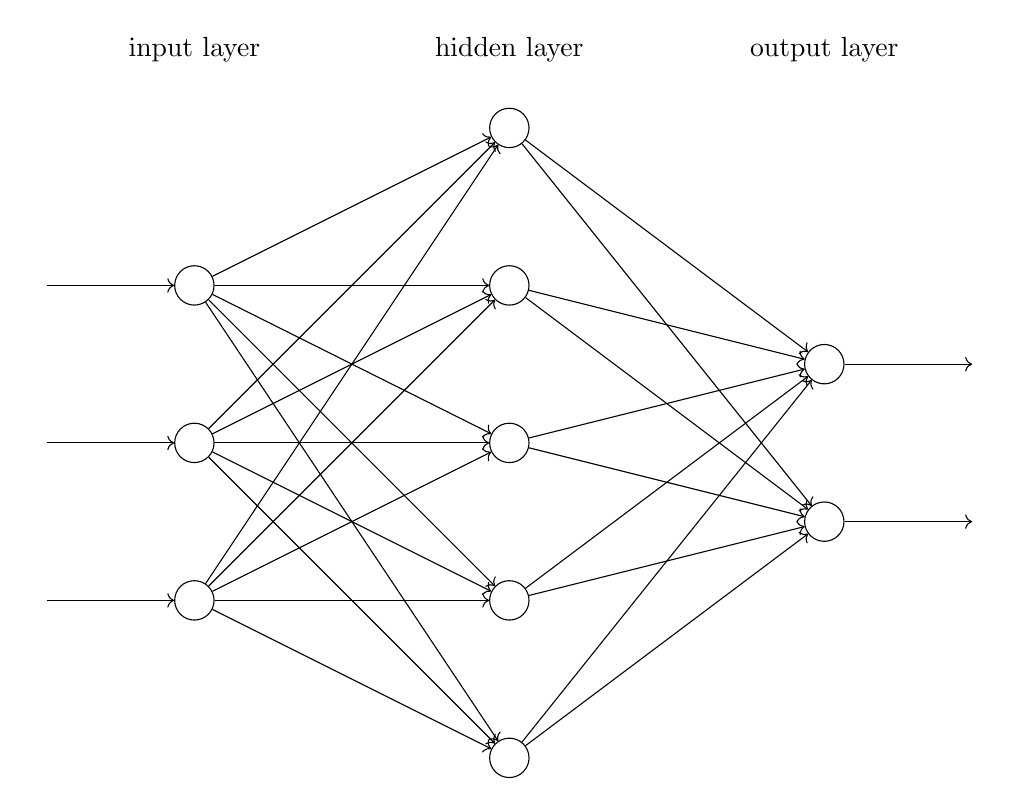
\begin{tikzpicture}[dot/.style={circle,draw,minimum size = .5cm}]
		\node at(-4,5) {input layer};
		\node at(0,5) {hidden layer};
		\node at(4,5) {output layer};

		\node at(6,1) (oo1) {};
		\node at(6,-1) (oo2) {};

		\node at (4,1) [dot] (o1) {}
			edge[->] (oo1);
		\node at (4,-1) [dot] (o2) {}
			edge[->] (oo2);

		\node at (0,4) [dot] (h1) {}
			edge[->] (o1)
			edge[->] (o2);
		\node at (0,2) [dot] (h2) {}
			edge[->] (o1)
			edge[->] (o2);
		\node at (0,0) [dot] (h3) {}
			edge[->] (o1)
			edge[->] (o2);
		\node at (0,-2) [dot] (h4) {}
			edge[->] (o1)
			edge[->] (o2);
		\node at (0,-4) [dot] (h5) {}
			edge[->] (o1)
			edge[->] (o2);

		\node at (-4,2) [dot] (i1) {}
			edge[->] (h1)
			edge[->] (h2)
			edge[->] (h3)
			edge[->] (h4)
			edge[->] (h5);
		\node at (-4,0) [dot] (i2) {}
			edge[->] (h1)
			edge[->] (h2)
			edge[->] (h3)
			edge[->] (h4)
			edge[->] (h5);
		\node at (-4,-2) [dot] (i3) {}
			edge[->] (h1)
			edge[->] (h2)
			edge[->] (h3)
			edge[->] (h4)
			edge[->] (h5);

		\node at(-6,2) (ii1) {}
			edge[->] (i1);
		\node at(-6,0) (ii2) {}
			edge[->] (i2);
		\node at(-6,-2) (ii3) {}
			edge[->] (i3);
	\end{tikzpicture}
\end{center}
\caption {Schema of a MLP or feedforward neural network.}
\label{fig:mlp}
\end{figure}

A MLP can also be represented as a statistical model
$f(\mathbf{x};\mathbf{\theta})$.
Computing $f(\mathbf{x})$---also called \textit{inference} or the
\textit{forward pass}---can be described as a layer-wise composition
of functions $f^{(1)}, f^{(2)}, \dots, f^{(l)}$, each function
$f^{(i)}, i < l$ being a hidden layer and $f^{(l)}$ being the output
layer.
The perceptron has the weight vector $\mathbf{w}$ and the bias
$b$ as its parameters (see Equation~\ref{eq:perceptron}).
The parameters of a layer is the combination of
$\mathbf{w}$ and $b$ for each of its perceptrons.
For example, if the first hidden layer contains $m$ perceptrons and
$\mathbf{x}$ is a $n$-vector, then the parameters of $f^{(1)}$ would
be a matrix $\mathbf{W}: n \times m$ and a $m$-vector $\mathbf{b}$.
The output of layer $f^{(1)}$ would be a $m$-vector computed as
follows:
\begin{align}
  f^{(1)}(\mathbf{x}; \mathbf{W}, \mathbf{b}) =
  g(\mathbf{x}^\top \mathbf{W} + \mathbf{b})^\top.
\end{align}
The second layer takes the output of the first and so forth.
The forward pass of the MLP is computed as:
\begin{align}
  y = f^{(l)}(f^{(l-1)}(\dots f^{(1)}(\mathbf{x}))).
\end{align}

The backpropagation algorithm is a way to train the parameters of a
MLP (or other deep learning models) so that it approximates the
unknown function $f^*$ which generates the labels of the examples
we have in our data set.
The data set used for training a model is called the \textit{training
set}. Additionally to the training set there normally exists a
\textit{test set} with examples the model has not seen before.
The test set is used to determine the generalization performance of
the model.
Backpropagation is an algorithm that allows to train a deep learning
model with \textit{(stochastic or batch) gradient descent}.
For example, $\hat{y} = f(\mathbf{x})$ and $y$ is the true label
($y$ and $\hat{y}$ are $k$-vectors), the error of $f$ is computed
using a \textit{loss function} $L$, for example mean squared error:
$1/k \sum_{i=1}^{k}(y_k - \hat{y}_k)^2$.
In order to get the gradients of the weights of the output layer
we calculate the derivative of the loss according to each weight
$w_{ij}$ in $\mathbf{W}$ with the chain rule:
\begin{align}
  \frac{\delta L}{\delta w_{ij}} =
    \frac{\delta L}{\delta g}
    \frac{\delta g}{\delta h}
    \frac{\delta h}{\delta w_{ij}},
\end{align}
$h$ being $f^{(l-1)\top}\mathbf{W} + \mathbf{b}$.
$w_{ij}$ is updated by performing the stochastic gradient descent%
\footnote{Or (batch) gradient descent. With gradient descend the whole
  training set is passed through the MLP before the weights
  are updated with the sum over the loss of each example in the
  training set. Batch or Mini-batch gradient descent takes a subset of
  the whole training set and updates the weights after each
  mini-batch. Deep learning models are normally trained by passing the
  training set multiple times through the model. Each pass over the
  whole training set is called an \textit{epoch}.
}:
\begin{align}
  w_{ij}^+ = w_{ij} - \mu \frac{\delta L}{\delta w_{ij}},
\end{align}
with $\mu$ as the \textit{learning rate}.
The same procedure is applied to the following hidden layers.
The total loss of the next hidden layer is given as:
\begin{align}
  L^{(l-1)} = \sum_{i=1}^n\frac{\delta L}{\delta f^{(l - 1)}_i} =
  \sum_{i=1}^n\frac{\delta L}{\delta g}
    \frac{\delta g}{\delta h}
    \frac{\delta h}{\delta f^{(l - 1)}_i},
\end{align}
$f^{(l-1)}_i$ being the $i$-th perceptron of the hidden layer $l-1$.

\citet{hornik_et_al_1989} demonstrated that a non-linear MLP
(the activation functions are non-linear transformations of
$h(x) = \mathbf{x}^\top \mathbf{W} + \mathbf{b}$) can overcome the
famous XOR problem of a single layer perceptron demonstrated in
\citet{minsky_et_al_1969}.
Another major contribution of the phase of connectionism was the
neocognitron \citep{fukushima_1980}, the origin of today's
\textit{convolutional neural networks} (CNNs)---which are the
state-of-the-art approach for building computer vision models---and
the application of the backpropagation algorithm to fully automate the
training of CNNs \citep{lecun_et_al_1989}.

\citet{goodfellow_et_al_2016} claims that the third and current phase
of deep learning---where the name deep learning was
established---starts with \citet{hinton_et_al_2006} describing a new
learning algorithm called greedy layer-wise pretraining, which they
applied to deep belief networks.
Greedy layer-wise pretraining was soon generalized to work with other
deep artificial neural network architectures
\citep{renzato_et_al_2006, bengio_et_al_2007}.
While these papers may have resulted in the term deep learning,
they were not the reason for the resurrected interest in this
methodology.
The two most important factors are the increase of available data
and computation.
The former enables better generalization while the latter allows
training bigger models (more hidden layers---the \textit{depth} of the
neural networks increased) which can solve more complex problems
\citep{goodfellow_et_al_2016}.

Like the perceptron, ``neurons'' in a \textit{convolutional layer}
are inspired by findings of neuroscientists.
In this case by research done by Hubel and Wiesel about the
mammalian visual cortex
\citep{hubel_et_al_1959, hubel_et_al_1962, hubel_et_al_1968}.
CNNs are just deep learning models which have at least one
convolutional layer. They are applied to problems which have a
grid-like topology, like time-series (1D), images (2D) or videos (3D)
\citep{goodfellow_et_al_2016}.

Unlike dense layers of perceptrons, convolutional layers do not apply
a full matrix multiplication $\mathbf{x}^\top\mathbf{W}$ but instead
a linear operation $*$ called convolution.
A one dimensional discrete convolution can be described as:
\begin{align}
  \label{eq:conv}
  s(i) = (x * w)(i) = \sum_n x(i + n)w(n).
\end{align}
Equation~\ref{eq:conv} is not really a convolution but is referred to
as \textit{cross-correlation}.
Unlike true convolution, cross-correlation is not commutative
\citep{goodfellow_et_al_2016}.
But commutativity is not a factor in practice, so many deep learning
libraries, like Keras \citep{keras} or the prototype developed for
this thesis implement cross-correlation rather than true convolution.
Below convolution will refer to cross-correlation.

In the case of deep learning, $x$ is a $n$D array called the
\textit{input} and $w$ is another $n$D array referred to as the
\textit{kernel}. The kernel elements are the trainable parameters
\citep{goodfellow_et_al_2016}.
In Equation~\ref{eq:conv}, $x$ and $w$ are one dimensional.
If we say $x$ to be a $m$-vector, the function $x(i)$ is defined as:
\begin{align}
  \label{eq:valid_conv}
  x(i) = \begin{cases}
    x_i &\text{if } 1 \leq i \leq m \\
    0 &\text{otherwise.}
  \end{cases}
\end{align}
$n$ is the size of the kernel in the first dimension.
Figure~\ref{fig:conv_op} shows an example of how the output of a
1D convolutional layer is computed.
Figure~\ref{fig:cnn} shows the schema of the convolutional
layer performing the operation from Figure~\ref{fig:conv_op}.
The result of a convolution can be transformed by an activation
function like the perceptron and the concept of the bias applies also.

\begin{figure}
\begin{center}
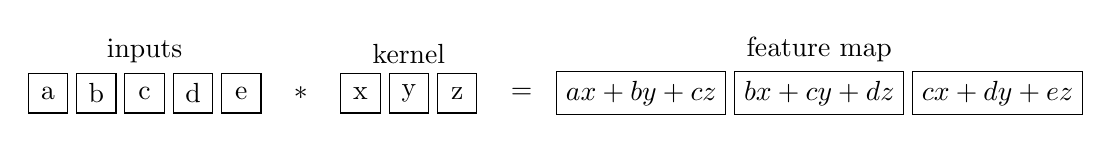
\begin{tikzpicture}[box/.style={rectangle,draw, minimum size=.5cm}]
  \node[box] at (0,0) (a) {a};
  \node[right=.1 of a, box] (b) {b};
  \node[right=.1 of b, box, label=inputs] (c) {c};
  \node[right=.1 of c, box] (d) {d};
  \node[right=.1 of d, box] (e) {e};

  \node[right=.9 of d] {$*$};

  \node[right=1 of e, box] (x) {x};
  \node[right=.1 of x, box, label=kernel] (y) {y};
  \node[right=.1 of y, box] (z) {z};

  \node[right=.3 of z] {$=$};

  \node[right=1 of z, box] (fst) {$ax + by + cz$};
  \node[right=.1 of fst, box, label=feature map] (snd)
    {$bx + cy + dz$};
  \node[right=.1 of snd, box] (trd) {$cx + dy + ez$};
\end{tikzpicture}
\end{center}
\caption{Example of a 1D cross-correlation operation with a kernel
  size of three, a single channel, a single filter, a stride of one
  and valid padding.}
\label{fig:conv_op}
\end{figure}

\begin{figure}
\begin{center}
	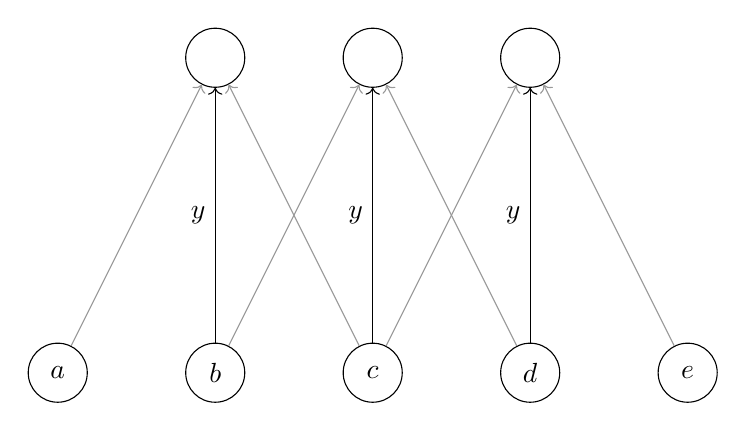
\begin{tikzpicture}[rotate=90, dot/.style={circle,draw,minimum size = .75cm}]
		\node at (0,2) [dot] (h2) {};
		\node at (0,0) [dot] (h3) {};
		\node at (0,-2) [dot] (h4) {};

		\node at (-4,4) [dot] (i1) {$a$}
			edge[black!40, ->] (h2);
		\node at (-4,2) [dot] (i2) {$b$}
			edge[->] (h2)
			edge[black!40, ->] (h3);
		\node at (-4,0) [dot] (i3) {$c$}
			edge[black!40, ->] (h2)
			edge[->] (h3)
			edge[black!40, ->] (h4);
		\node at (-4,-2) [dot] (i4) {$d$}
			edge[black!40, ->] (h3)
			edge[->] (h4);
		\node at (-4,-4) [dot] (i5) {$e$}
			edge[black!40, ->] (h4);

    \node[left] at (-2,2) {$y$};
    \node[left] at (-2,0) {$y$};
    \node[left] at (-2,-2) {$y$};
	\end{tikzpicture}
\end{center}
\caption {Schema for the convolutional layer performing the
  convolution shown in Figure~\ref{fig:conv_op}. Each neuron
  represents one convolution. The schema shows the
  property of shared weights and sparse
  connectivity \citep{goodfellow_et_al_2016}. The black edges
  all have the same associated weight $y$, while one can see that
  there are much less edges compared to a dense layer shown in
  Figure~\ref{fig:mlp}.}
\label{fig:cnn}
\end{figure}

Normally a convolutional layer does not consist of a single
convolution, but applies multiple kernels to the output of the
previous layer.
A single convolution is called a \textit{filter} and a layer
consists of a predefined amount of filters, each with its own kernel
\citep{brownlee_2019}.
The output of a convolutional layer is often called a
\textit{feature map} \citep{goodfellow_et_al_2016}.
Even though an image may seem to be a two dimensional structure of
pixels, in most cases it is actually three dimensional, the third
dimension being the RGB color values for each pixel.
The third dimension of the three RGB colors are called the
\textit{channels} \citep{goodfellow_et_al_2016}.
For example, we have a data set of images with $256\times256$
pixels and three channels (red, green and blue).
We pass the image to a convolutional layer with a $3\times3$ kernel
shape and $64$ filters.
A kernel consists of 18 elements, the kernel size (for the two
spatial dimensions) times the three channels of each pixel.
The shape of the feature map of that layer---if we assume ``same''
padding (see below)---would be $256\times256\times64$, so the
next layer would have 64 channels.

There are two more notable concepts of convolutional layers:
\textit{stride} and \textit{padding}.
The former refers to skipping convolutions in order to reduce the
computational cost at the expense of less exact feature extraction
(patterns may not be detected by the model due to the increased
inaccuracy).
The latter is a way of dealing with vanishing spacial dimensions of
the feature map if we only perform convolutions on ``valid'' inputs
($1 \leq i \leq m$ in Equation~\ref{eq:valid_conv}).
``valid'' padding refers to the fact that the input has no padding,
which means the feature map of the convolutional layer will have
its kernel size minus one less neurons than its input
(see Figure~\ref{fig:cnn}).
``Same'' padding would be to add enough zeros evenly above and below
the valid input (along each spacial dimension) so that the feature map
of the convolutional layer will have the same spacial dimensions as
its input (see Figure~\ref{fig:padding} \citep{goodfellow_et_al_2016}.

\begin{figure}
\begin{center}
	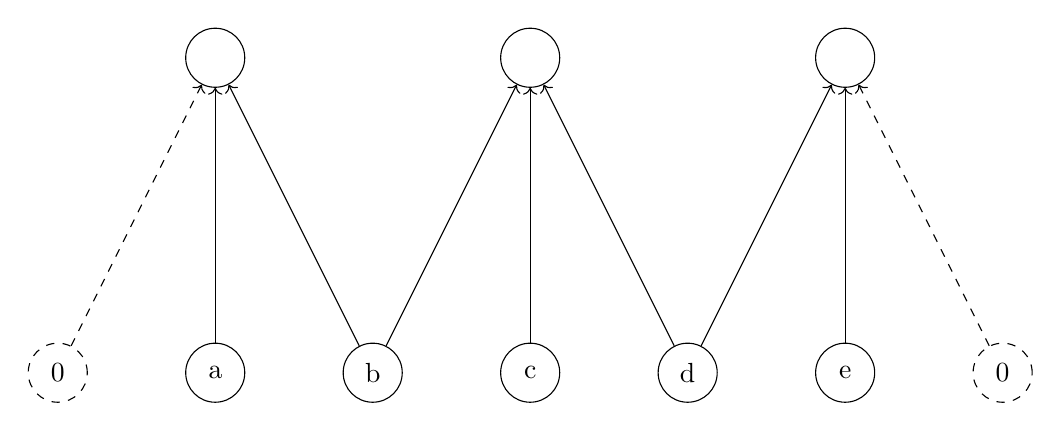
\begin{tikzpicture}[rotate=90, dot/.style={circle,draw,minimum size = .75cm}]
		\node at (0,4) [dot] (h1) {};
		\node at (0,0) [dot] (h3) {};
		\node at (0,-4) [dot] (h5) {};

		\node at (-4,6) [dot, dashed] (i0) {0}
			edge[->, dashed] (h1);
		\node at (-4,4) [dot] (i1) {a}
      edge[->] (h1);
		\node at (-4,2) [dot] (i2) {b}
			edge[->] (h1)
			edge[->] (h3);
		\node at (-4,0) [dot] (i3) {c}
			edge[->] (h3);
		\node at (-4,-2) [dot] (i4) {d}
			edge[->] (h3)
			edge[->] (h5);
		\node at (-4,-4) [dot] (i5) {e}
			edge[->] (h5);
		\node at (-4,-6) [dot, dashed] (i6) {0}
			edge[->, dashed] (h5);
	\end{tikzpicture}
\end{center}
\caption {Example showing a layer with same padding and a
  stride of two.}
\label{fig:padding}
\end{figure}

Along convolutional layers, CNNs often have \textit{pooling layers}.
A pooling layer summarizes locally with the goal of making the
CNN invariant to small translations of the input
\citep{goodfellow_et_al_2016}, making the model less prone to
\textit{overfitting}---the state a model is in if it performs well
on the training set but does not generalize well to unseen examples
(bad performance on the test set).
\textit{Max pooling}, for example, takes some local neighborhood of
the input, exactly like a convolutional layer, and returns the
maximum value of that neighborhood.

% }}}

\subsection{Benchmarking Deep Learning Systems for Computer Vision} % {{{
\label{subsec:intro_bench}

In 2010 the annual (until 2017) ImageNet Large Scale Visual
Recognition Challenge (ILSVRC) was launched and has become the most
famous benchmark for computer vision models, producing many well-known
deep learning models like AlexNet in 2012
\citep{krizhevsky_et_al_2012}, VGG16 in 2014
\citep{simonyan_et_al_2014} and the ResNet models in 2015
\citep{he_et_al_2015}.
The ILSVRC---like the name suggests---is based on the ImageNet data
set consisting of more than 14 million images
\citep{russakovsky_et_al_2015}.
One task of the ILSVRC benchmark is image classification.
During image classification the model is trained on 1000 categories
(1.2 million images), without overlapping labels (each image has a
single label, e.g.~``dog'') \citep{russakovsky_et_al_2015}.
The top-1 ($y = \text{argmax } f(\mathbf{x})$) accuracy is measured on
a test set of 150,000 images and winner is the model with the highest
top-1 accuracy.

While a benchmark like the ILSVRC produces new insights into computer
vision and keeps the community up-to-date on what is possible,
deep learning has another issue on which a benchmark can shed light:
training/inference speed of hardware and software systems.
The MLPerf benchmark was developed to tackle this problem, so
stakeholders can make informed decisions and to provide the
industry---like hardware vendors, cloud providers and machine learning
engineers---with a fair standard to rely on
\citep{mattson_et_al_2019}.
One task of the MLPerf training benchmark is training the ResNet-50
model (see below) on the image classification task from the ILSVRC
2012, until it reaches a top-1 accuracy of 74.9 percent.
The wallclock time is measured and serves as the result for the
benchmarked system \citep{mattson_et_al_2019}.
Currently the fastest solution, from the latest MLPerf training
benchmark v0.6, is Google's cloud system based on Tensorflow and
one TPUv3 pod (1024 TPUv3s) \citep{mlperf_2019, stone_2019}.
Our benchmark presented in Section~\ref{sec:benchmark} will be based
on the image classification task of the MLPerf training benchmark,
making it easy to compare SpiNNaker and our prototype to other
state-of-the-art deep learning systems.

Winner of the image classification task of the ILSVRC 2015 was an
ensemble of residual nets (ResNets) introduced in
\citet{he_et_al_2015}.
The ensemble generated a top-5 accuracy (true label in the five
highest outputs of the ensemble) of 96.4 percent.
ResNets are a revolution in the sense that they are not only better
classifiers than previous models, they also can be significantly
deeper \citep{he_et_al_2015}.
\citet{he_et_al_2015} presents a 152-layer deep network, eight times
deeper than a ``very deep convolutional network'' (VGG11--VGG19)
\citep{simonyan_et_al_2014, he_et_al_2015}.
ResNets can be so deep, without losing their ability of convergence
and without degradation (saturated accuracy and higher training error
with increased depth) \citep{he_et_al_2015}, by introducing residual
blocks with shortcut connections (see Figure~\ref{fig:shortcut_conn}).
\citet{he_et_al_2015} hypothesizes that residual blocks ease the
learning of the model.
These shortcut connections do not increase the complexity of the
model. No additional parameters are added to the model and nothing
changes during backpropagation.
Only the negligible operation where $\mathbf{x}$ is added to the
output of the residual block must be performed during the forward
pass.
\citet{he_et_al_2015} shows comprehensive tests on how residual blocks
decrease degradation impact by comparing ResNets against their
counterpart with the same architecture, but without shortcut
connections.
The models without shortcut connections show a higher training error
than their ResNet counterpart.

\begin{figure}
  \begin{center}
    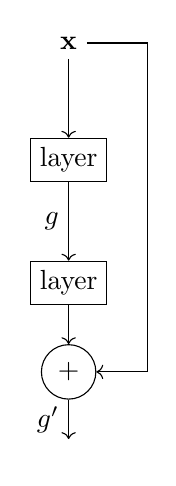
\begin{tikzpicture}
      \node[rectangle, draw] at (0, 0) (layer0) {layer};
      \node[rectangle, draw, below=1 of layer0] (layer1) {layer};
      \node[circle, draw, below=.5 of layer1] (layer_add) {$+$};
      \node[below=.5 of layer_add] (layer_out) {};
      \node[above=1 of layer0] (layer_in) {$\mathbf{x}$};

      \draw[->] (layer_in) -- (layer0);
      \draw[->] (layer0) -- node[left]{$g$} (layer1);
      \draw[->] (layer1) -- (layer_add);
      \draw[->] (layer_add) -- node[left]{$g^\prime$} (layer_out);

      \draw[->] (layer_in) -| ($(layer_add) + (1,0)$) |- (layer_add);
    \end{tikzpicture}
  \end{center}
  \caption{Schema of a residual block with two layers. $\mathbf{x}$ is
    added to the output of the last layer of the residual block,
    before the result is passed through its activation function
    $g^\prime$.}
  \label{fig:shortcut_conn}
\end{figure}

Like stated above, the image classification task of the MLPerf
training benchmark is to train ResNet-50 (50, because it has 50
layers) until it reaches a top-1 accuracy of 74.9 percent on the test
set and to measure the wallclock time it took to reach that goal.
Figure~\ref{fig:resnet50_block} shows an example block from the
ResNet-50 model, while Figure~\ref{fig:resnet50} shows its
architecture.

\begin{figure}
  \begin{center}
    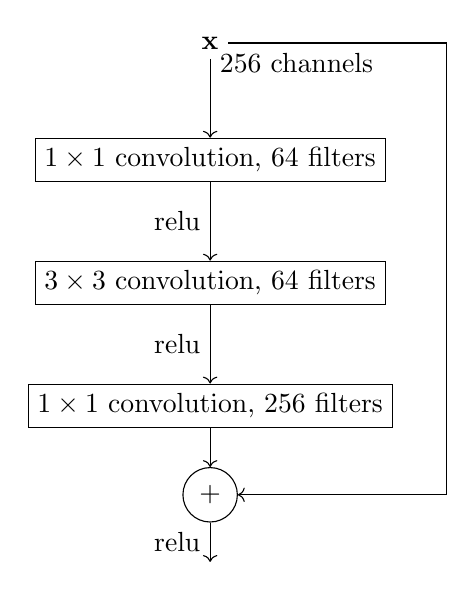
\begin{tikzpicture}
      \node[rectangle, draw] at (0, 0) (layer0)
        {$1\times1$ convolution, 64 filters};
      \node[rectangle, draw, below=1 of layer0] (layer1)
        {$3\times3$ convolution, 64 filters};
      \node[rectangle, draw, below=1 of layer1] (layer2)
        {$1\times1$ convolution, 256 filters};
      \node[circle, draw, below=.5 of layer2] (layer_add) {$+$};
      \node[below=.5 of layer_add] (layer_out) {};
      \node[above=1 of layer0] (layer_in)
        {$\mathbf{x}$};

      \draw[->] (layer_in) -- (layer0);
      \draw[->] (layer0) -- node[left]{relu} (layer1);
      \draw[->] (layer1) -- node[left]{relu} (layer2);
      \draw[->] (layer2) -- (layer_add);
      \draw[->] (layer_add) -- node[left]{relu} (layer_out);

      \draw[->] (layer_in) node[below right] {256 channels} -| ($(layer_add) + (3,0)$) |- (layer_add);
    \end{tikzpicture}
  \end{center}
  \caption{Example of a residual block in ResNet-50.}
  \label{fig:resnet50_block}
\end{figure}

\begin{figure}
  \begin{center}
    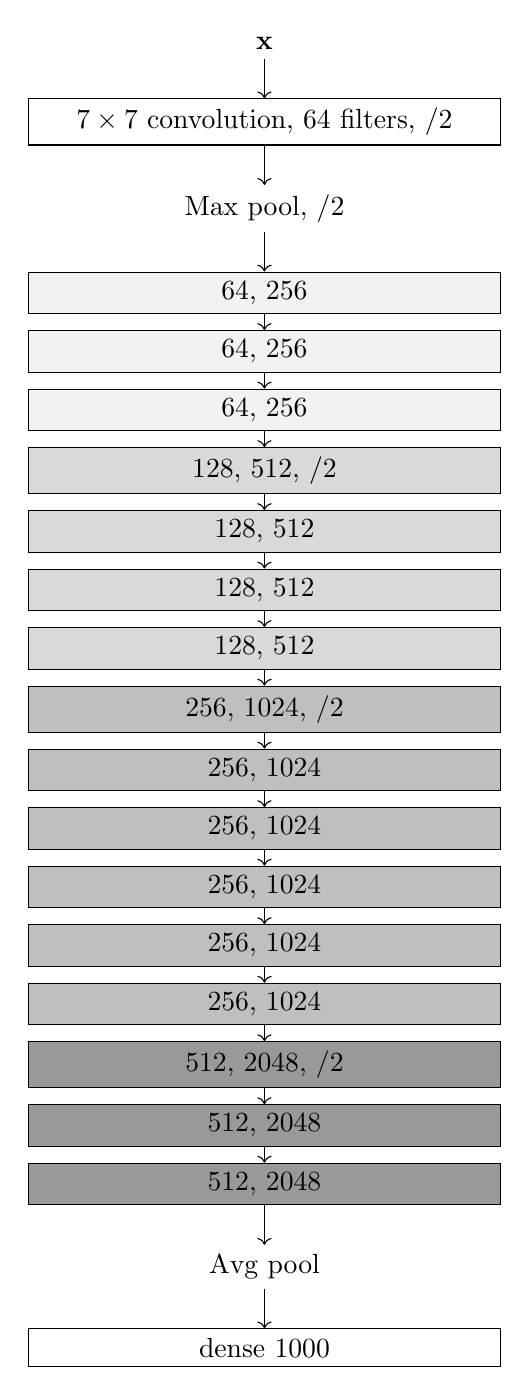
\begin{tikzpicture}[block/.style={rectangle, draw, minimum width=6cm}]
      \node[block, fill=black!5] at (0, 0) (block0) {64, 256};
      \node[block, fill=black!5, below=.2 of block0] (block1) {64, 256};
      \node[block, fill=black!5, below=.2 of block1] (block2) {64, 256};

      \node[block, fill=black!15, below=.2 of block2] (block3) {128, 512, /2};
      \node[block, fill=black!15, below=.2 of block3] (block4) {128, 512};
      \node[block, fill=black!15, below=.2 of block4] (block5) {128, 512};
      \node[block, fill=black!15, below=.2 of block5] (block6) {128, 512};

      \node[block, fill=black!25, below=.2 of block6] (block7) {256, 1024, /2};
      \node[block, fill=black!25, below=.2 of block7] (block8) {256, 1024};
      \node[block, fill=black!25, below=.2 of block8] (block9) {256, 1024};
      \node[block, fill=black!25, below=.2 of block9] (block10) {256, 1024};
      \node[block, fill=black!25, below=.2 of block10] (block11) {256, 1024};
      \node[block, fill=black!25, below=.2 of block11] (block12) {256, 1024};

      \node[block, fill=black!40, below=.2 of block12] (block13) {512, 2048, /2};
      \node[block, fill=black!40, below=.2 of block13] (block14) {512, 2048};
      \node[block, fill=black!40, below=.2 of block14] (block15) {512, 2048};

      \node[below=.5 of block15] (pool2) {Avg pool};
      \node[block, below=.5 of pool2] (dense) {dense 1000};

      \node[above=.5 of block0] (pool1) {Max pool, /2};
      \node[block, above=.5 of pool1] (conv1)
        {$7\times7$ convolution, 64 filters, /2};
      \node[above=.5 of conv1] (x) {$\mathbf{x}$};

      \draw[->] (block0) -- (block1);
      \draw[->] (block1) -- (block2);
      \draw[->] (block2) -- (block3);
      \draw[->] (block3) -- (block4);
      \draw[->] (block4) -- (block5);
      \draw[->] (block5) -- (block6);
      \draw[->] (block6) -- (block7);
      \draw[->] (block7) -- (block8);
      \draw[->] (block8) -- (block9);
      \draw[->] (block9) -- (block10);
      \draw[->] (block10) -- (block11);
      \draw[->] (block11) -- (block12);
      \draw[->] (block12) -- (block13);
      \draw[->] (block13) -- (block14);
      \draw[->] (block14) -- (block15);

      \draw[->] (x) -- (conv1);
      \draw[->] (conv1) -- (pool1);
      \draw[->] (pool1) -- (block0);
      \draw[->] (block15) -- (pool2);
      \draw[->] (pool2) -- (dense);
    \end{tikzpicture}
  \end{center}
  \caption{Schema of ResNet-50. Each block in the middle represents
    one residual block shown in Figure~\ref{fig:resnet50_block}.
    The first number shows the amount of filters the first two layers
    of a block have, while the second number shows the filters of the
    last layer of the block. $/2$ indicates that a stride of two is
    applied (spacial dimensions are halved---each convolutional and
    pooling layer has ``same'' padding). Whenever the filters are
    doubled (indicated by the varying grey scales), the shortcut layer
    is linearly projected to match the higher channels.}
  \label{fig:resnet50}
\end{figure}

% }}}

\subsection{SpiNNaker as a Neuromorphic Computer Architecture} % {{{
\label{subsec:intro_spinn}

\begin{enumerate}
  \item describe spinnaker and the spinnaker architecture
  \item compare to other DL accelerators (GPGPUs and TPUs)
\end{enumerate}
% spinnaker architecture

% compare to other state of the art machine learning hardware

% why didn't we just implement a backend (e.g. tensorflow?)
% because architecture is so different (MACs vs. massive parallelism
% with small messages)

% }}}

% }}}


\section{Related Work} % {{{
\label{sec:related_work}

\begin{enumerate}
  \item SNNToolbox for translating DNNs to SNNs (only inference)
  \item TrueNorth has a paper about its DL implementation
  \item (optional) The 2011 paper about mapping MLP's and recurrent
    networks onto SpiNNaker
\end{enumerate}

% }}}


\section{Deep Learning on SpiNNaker}
\label{sec:SpiDNN}

\begin{itemize}
  \item concepts (layers, neurons, \dots)
  \item partitions and how that allows me to use min keys to discern
    between what I have received
  \item communication structure (partitions and global partition manager)
  \item ping-pong
  \item graph structure (especially focused on edge and host--SpiNN
    communication)
  \item interpreting neurons as domain decomposition over linear algebra
    compute graph
  \item backward pass: gradients computed two times so comm fabric is
    not overly used by unique partitions/lots of unused packages
  \item How I crushed $n$d-kernels into a single blog of weights (same
    for 2D convolutions even though less interesting)
\end{itemize}

\section{Benchmark}
\label{sec:benchmark}

\section{Discussion}
\label{sec:discussion}

\begin{itemize}
  \item space used inefficiently (cores and memory) $\rightarrow$ better
    domain decomposition
  \item batch normalization and their implications for
    vanishing/exploding gradients
\end{itemize}

\section{Conclusion}
\label{sec:conclusion}

\section{Next Steps}
\label{sec:next_steps}

\begin{itemize}
  \item profiling
  \item cost model
  \item multiple copies of the same network on the same machine
    $\rightarrow$ use all resources available
  \item better domain decomposition (SpiNNaker application graph or
    custom solution (application graph not helpful for neurons which
    become too big))
  \item smart algorithms vs.\ integrating with state-of-the-art libraries
    (investing time in stuff like SLIDE and the one paper by the Austrian
    guys about sparse connections explicitly mentioning SpiNNaker and
    neuromorphic chips or rather work on a trans-/compiler
    that efficiently translates linear algebra operations (like TF,
    PyTorch,\dots) onto SpiNNaker)
  \item integrate into compiler projects like Apache-TVM, XLA, Glow,
   nGraph, etc.
  \item implementing ONNX spec to make it easy for developers to use
    SpiNNaker (develop in PyTorch $\rightarrow$ run on SpiNNaker)
\end{itemize}

\bibliography{library.bib}
\addcontentsline{toc}{section}{References}

\end{document}
